\documentclass[tikz, border=15pt]{standalone}
\usepackage{tikz}
\usetikzlibrary{calc, arrows.meta, positioning}

\definecolor{basecolor}{HTML}{2B6CB0}
\definecolor{jointcolor}{HTML}{ED8936}
\definecolor{linkcolor}{HTML}{CBD5E0}
\definecolor{darklink}{HTML}{718096}
\definecolor{grippercolor}{HTML}{E53E3E}

\begin{document}
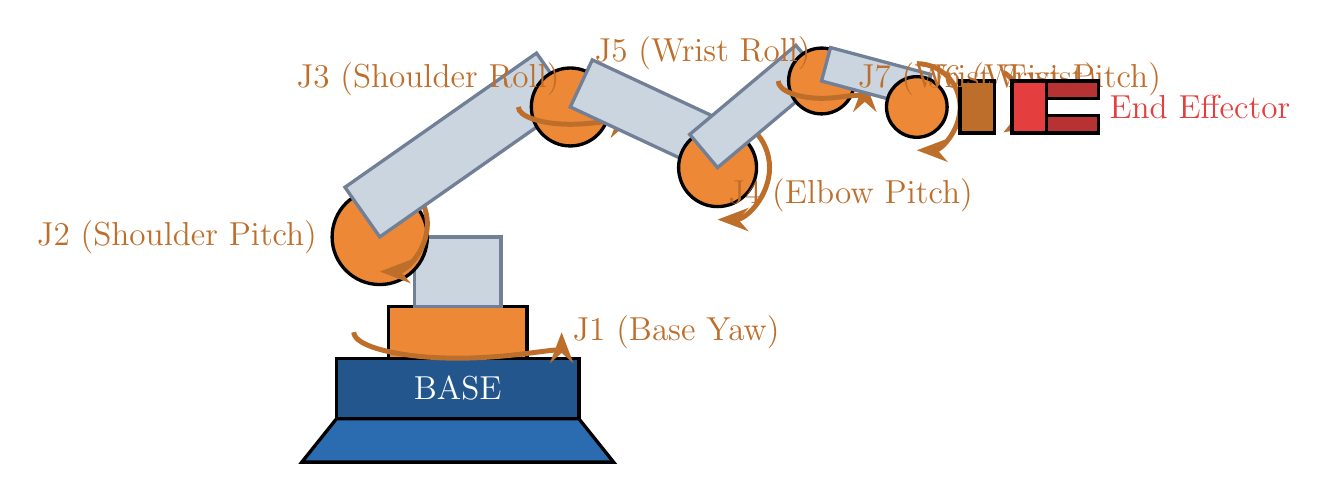
\begin{tikzpicture}[
    scale=1.1,
    >=Stealth,
    line width=1.2pt,
    font=\sffamily\bfseries
]

    % Base Platform (J1 Base)
    \fill[basecolor, draw=black] (-1.8, -3.0) -- (1.8, -3.0) -- (1.4, -2.5) -- (-1.4, -2.5) -- cycle;
    \fill[basecolor!80!black, draw=black] (-1.4, -2.5) rectangle (1.4, -1.8);
    \node[white, font=\large] at (0, -2.15) {BASE};

    % Joint 1 (J1: Base Rotation - Yaw)
    \fill[jointcolor, draw=black] (-0.8, -1.8) rectangle (0.8, -1.2);
    \draw[->, line width=1.8pt, jointcolor!80!black] (-1.2, -1.5) arc (180:360:1.2 and 0.3);
    \node[right, jointcolor!80!black, font=\large] at (1.2, -1.5) {J1 (Base Yaw)};

    % Link 1
    \fill[linkcolor, draw=darklink] (-0.5, -1.2) rectangle (0.5, -0.4);

    % Joint 2 (J2: Shoulder Pitch)
    \fill[jointcolor, draw=black] (-0.9, -0.4) circle (0.55);
    \draw[->, line width=1.8pt, jointcolor!80!black] (-0.9, 0.3) arc (90:-90:0.55);
    \node[left, jointcolor!80!black, font=\large] at (-1.5, -0.4) {J2 (Shoulder Pitch)};

    % Link 2 (Upper Arm going up-right)
    \fill[linkcolor, draw=darklink, rotate around={35:(-0.9,-0.4)}] (-0.9, -0.4) rectangle (1.8, 0.3);

    % Joint 3 (J3: Shoulder Roll)
    \coordinate (J3pos) at (1.3, 1.1);
    \fill[jointcolor, draw=black] (J3pos) circle (0.45);
    \draw[->, line width=1.8pt, jointcolor!80!black] (J3pos) ++(-0.6, 0) arc (180:360:0.6 and 0.2);
    \node[above left, jointcolor!80!black, font=\large] at (J3pos) {J3 (Shoulder Roll)};

    % Link 3 (Elbow Link)
    \fill[linkcolor, draw=darklink, rotate around={-25:(J3pos)}] (J3pos) rectangle ++(1.8, 0.6);

    % Joint 4 (J4: Elbow Pitch)
    \coordinate (J4pos) at (3.0, 0.4);
    \fill[jointcolor, draw=black] (J4pos) circle (0.45);
    \draw[->, line width=1.8pt, jointcolor!80!black] (J4pos) ++(0, 0.6) arc (90:-90:0.6);
    \node[below right, jointcolor!80!black, font=\large] at (J4pos) {J4 (Elbow Pitch)};

    % Link 4 (Forearm Link going up-right)
    \fill[linkcolor, draw=darklink, rotate around={40:(J4pos)}] (J4pos) rectangle ++(1.6, 0.5);

    % Joint 5 (J5: Wrist Roll)
    \coordinate (J5pos) at (4.2, 1.4);
    \fill[jointcolor, draw=black] (J5pos) circle (0.38);
    \draw[->, line width=1.8pt, jointcolor!80!black] (J5pos) ++(-0.5, 0) arc (180:360:0.5 and 0.2);
    \node[above left, jointcolor!80!black, font=\large] at (J5pos) {J5 (Wrist Roll)};

    % Link 5
    \fill[linkcolor, draw=darklink, rotate around={-15:(J5pos)}] (J5pos) rectangle ++(1.2, 0.4);

    % Joint 6 (J6: Wrist Pitch)
    \coordinate (J6pos) at (5.3, 1.1);
    \fill[jointcolor, draw=black] (J6pos) circle (0.35);
    \draw[->, line width=1.8pt, jointcolor!80!black] (J6pos) ++(0, 0.5) arc (90:-90:0.5);
    \node[above right, jointcolor!80!black, font=\large] at (J6pos) {J6 (Wrist Pitch)};

    % Joint 7 (J7: Wrist Twist / Flange)
    \coordinate (J7pos) at (6.0, 1.1);
    \fill[jointcolor!80!black, draw=black] (J7pos) ++(-0.2,-0.3) rectangle ++(0.4, 0.6);
    \draw[->, line width=1.8pt, jointcolor!80!black] (J7pos) ++(0.3, 0.4) arc (60:-60:0.4);
    \node[above, jointcolor!80!black, font=\large] at (J7pos) {J7 (Wrist Twist)};

    % End Effector Gripper
    \fill[grippercolor, draw=black] (6.4, 0.8) rectangle (6.8, 1.4);
    \fill[grippercolor!80!black, draw=black] (6.8, 1.2) rectangle (7.4, 1.4); % Top finger
    \fill[grippercolor!80!black, draw=black] (6.8, 0.8) rectangle (7.4, 1.0); % Bottom finger
    \node[right, grippercolor, font=\large] at (7.4, 1.1) {End Effector};

\end{tikzpicture}
\end{document}
